% Approved figure placements for the V0.8 draft.
% Keep these widths synchronized with the paper source.

\begin{figure*}[t]
\centering
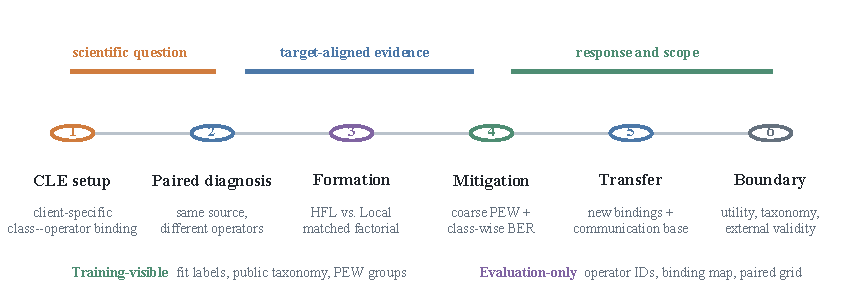
\includegraphics[width=0.94\textwidth,keepaspectratio]{figures/fig1_cle_hfl_evidence_chain.pdf}
\caption{CLE-HFL evidence chain and information boundary.}
\label{fig:evidence-chain}
\end{figure*}

\begin{figure*}[t]
\centering
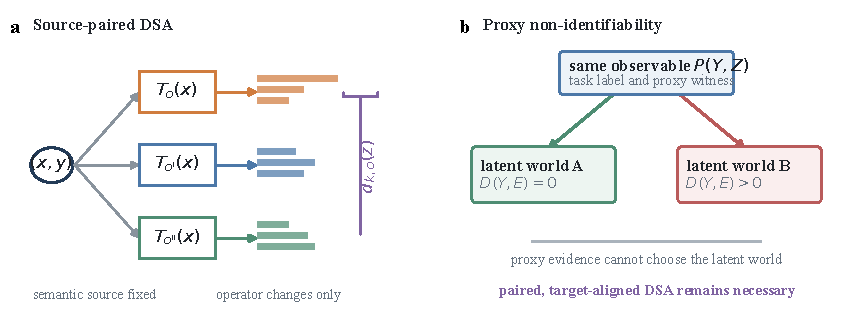
\includegraphics[width=0.94\textwidth,keepaspectratio]{figures/fig2_dsa_proxy_boundary.pdf}
\caption{Paired DSA and the proxy-identifiability boundary.}
\label{fig:dsa-proxy}
\end{figure*}

\begin{figure*}[t]
\centering
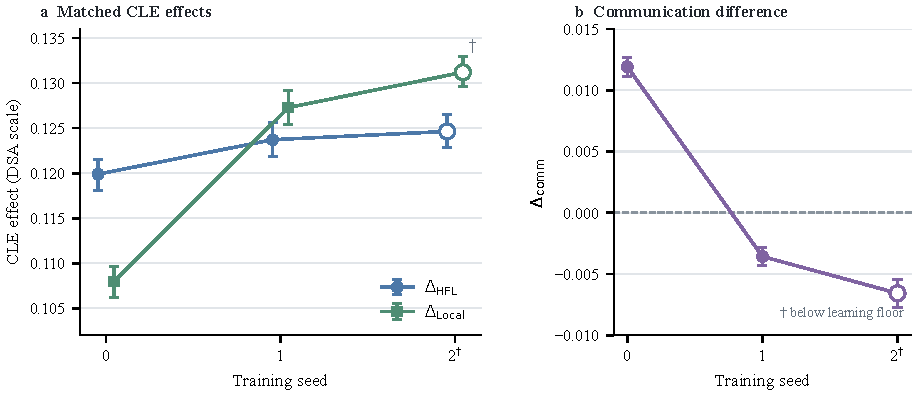
\includegraphics[width=0.92\textwidth,keepaspectratio]{figures/fig3_local_first_attribution.pdf}
\caption{DSA-based local-first formation across training seeds. Error bars are source-clustered 95\% intervals conditional on each trained checkpoint.}
\label{fig:local-first}
\end{figure*}

\begin{figure*}[t]
\centering
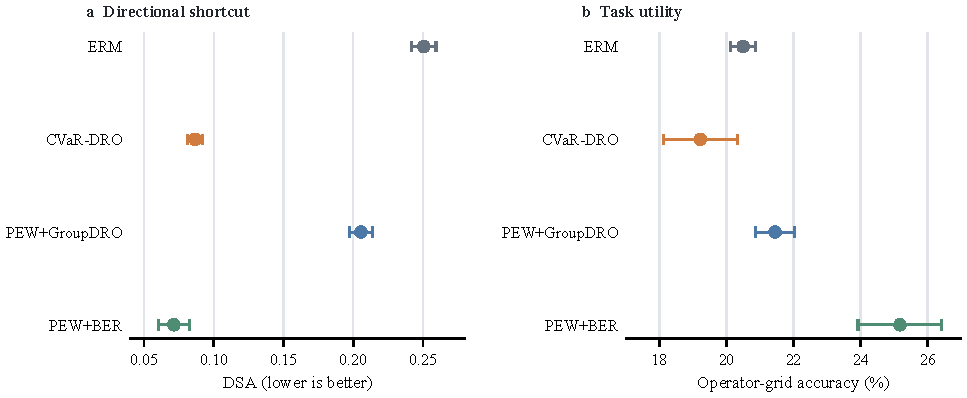
\includegraphics[width=0.90\textwidth,keepaspectratio]{figures/fig4_axis1_objective_comparison.pdf}
\caption{Fixed-budget matched objective comparison.}
\label{fig:axis1-objectives}
\end{figure*}

\begin{figure*}[t]
\centering
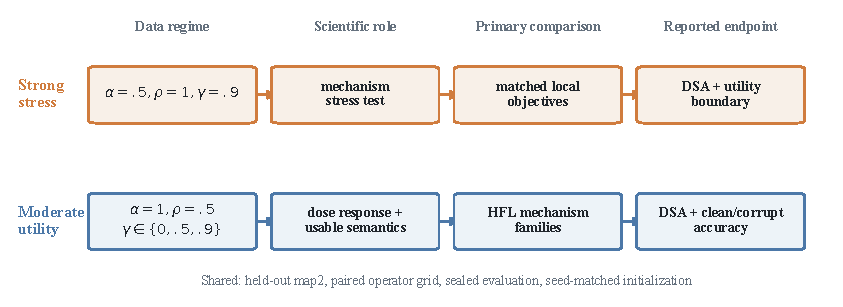
\includegraphics[width=0.94\textwidth,keepaspectratio]{figures/fig5_protocol_map.pdf}
\caption{Strong-stress and moderate-utility protocol roles.}
\label{fig:protocol-map}
\end{figure*}
